\chapter{Infraestructura}\label{cap.infraestructura}
En este capítulo tratará de abordar todos los componentes y software que han servido de apoyo en el desarrollo del TFG. En este punto daremos una explicación detallada sobre las plataformas en las que se cimienta el trabajo (ROS y JdeRobot), en el simulador Gazebo, en los editores de modelos, en las librerías más importantes (OpenCV y PyQt), en el proyecto Jupyter y en el entorno JdeRobot-Academy-Web.

\section{Entorno ROS}
ROS (Robot Operating System) proporciona a los desarrolladores de software robótico los componentes necesarios para el desarrollo de aplicaciones robóticas. Entre ellos destacan la abstracción hardware, bibliotecas, intercambios de mensajes, administración de paquetes, controladores de dispositivo y visualizadores. Esta plataforma se distribuye en código abierto bajo una licencia BSD.

Una de las características más importantes de ROS es su integración con el simulador Gazebo, con el que se comunica a través de paquetes llamados \textit{gazebo\_ros\_pkgs} \footnote{\url{http://ros.org/wiki/gazebo\_ros\_pkgs}}. Mediante estos paquetes, ROS es capaz de proporcionar las interfaces necesarias para simular un robot en Gazebo usando \textit{ROS Messages}, servicios y reconfiguración mecánica.

Esta plataforma se conforma como una colección de nodos o procesos que suponen una computación. Los nodos se combinan en un gráfico y se comunican entre sí mediante \textit{topics} de transmisión, servicios RPC y el Servidor de Parámetros. Un sistema de control de un robot se formará por la integración de distintos nodos, cuanto mayor sea la funcionalidad de la que se dote al robo, mayor número de nodos tendrá. Existen nodos de control de láser, vista gráfica del sistema, motores de ruedas, odometría, cámaras, etc. La existencia de nodos de ROS en el robot proporciona beneficios para el sistema robótico como tolerancia adicional a fallos soportados por cada nodo de manera indivual, de esta manera el fallo se concentra en un solo nodo. Además, la complejidad del código se reduce con los sistemas monolíticos.

Los \textit{topics} de ROS actúan como forma de comunicación, de esta manera se definen como buses sobre los que los nodos intercambian mensajes. Gracias a la semántica de publicación y/o suscripción anónima de los \textit{topics}, se desacopla la producción de información de consumo. Debido a esto los nodos no saben con quién se están comunicando. Por otra parte, los nodos interesados en un \textit{topic}, se suscriben a él para recoger la información que se publique por el mismo y, por otra parte, los nodos que generen datos pertenecientes a ese \textit{topic}, transmitirán la información por él. Es importante destacar que puede haber varios editores o generadores y varios suscriptores del mismo \textit{topic}.

Debido a la compatibilidad de ROS con Gazebo y con JdeRobot, se pueden utilizar los \textit{plugins} de ROS para las simulaciones en Gazebo de las prácticas presentes en el entorno JdeRobot mediante el establecimiento de las conexiones de los sensores y actuadores de la práctica con los \textit{plugins} de ROS en el nodo académico de la misma.

Existen una gran cantidad de \textit{plugins} de ROS que proporcionan una enorme diversidad de funcionalidad para el desarrollo de robots \footnote{\url{http://wiki.ros.org/gazebo_plugins}}. Entre ellos destacan el plugin que controla el láser, llamado \textit{libgazebo\_ros\_laser} o el que controla una cámara, llamado \textit{libgazebo\_ros\_camera}. Ambos plugins serán usados en las prácticas contenidas en este Trabajo de Fin de Grado.

\section{JdeRobot}
La plataforma \textit{JdeRobot}\footnote{\url{http://jderobot.org}} es un \textit{middleware} abierto para desarrolladores de robots y visión artificial. Fue creada por el Grupo de Robótica de la Universidad Rey Juan Carlos en 2003 y está licenciada como GPLv3\footnote{\url{https://www.gnu.org/licenses/quick-guide-gplv3.html}}.
La estructura de esta plataforma ha sido desarrollada en C y C++, aunque tiene componentes escritos en Python y JavaScript. El entorno ofrecido es mediante componentes, los cuales son ejecutados como procesos que interoperan entre sí mediante \textit{middleware} de comunicaciones como ICE o \textit{ROS-Messages}, que permiten la interoperación de componente en un entorno multilenguaje.

JdeRobot facilita los \textit{drivers} necesarios para la funcionalidad de sus robots. De esta manera, los \textit{dirvers} están asociados al hardware del robot proporcionando interfaces de acceso, por lo que simplifica la comunicación de las aplicaciones con los actuadores del robot que se realiza mediante una función mediante los interfaces ICE o ROS.

Los dispositivos que se pueden encontrar en JdeRobot son muy diversos, destacan el cuadricópteros como el Ardronde de Parrot, operativo con ICE, o el SoloDrone de 3DR, operativo con ROS, los coches Fórmula1 desarrollados por la propia plataforma JdeRobot que incluyen modelos de la mayoría de las escuderías presentes en la Fórmula 1, operativos con ROS y modificados en este TFG para incluirlos en la plataforma. También se incluyen modelos como el boto Kobuki de Yujin Robot, el humanoide NAO de Aldebaran Robotics, cámaras fireware, USB e IP, los simuladores Stage y Gazebo, escáneres láser LMS de SICK y URG de Hokuyo, sensores de profundidad como Kinect y otros dispositivos X10 de domótica o \textit{drivers} específicos de control de cámaras, láser y motores de movimiento.

JdeRobot incorpora librerías de software libre para su uso como OpenCV para visión, Eligen para álgebra o PCL para manejo de nubes de puntos. Al ser compatible con ROS, en específico con ROS-Kinetic, las aplicaciones de la plataforma pueden incorporar nodos de ROS y conectarse a ellos de manera fluida.

Las prácticas que componen este Trabajo de Fin de Grado se han desarrollado en la versión de JdeRobot 5.6.2, última versión estable.

\section{Simulador Gazebo}
Gazebo\footnote{\url{http://gazebosim.org/}} es un simulador de robótica que permite emular escenarios tridimensionales para robots autónomos (Figura 3.1). Es apropiado para comprobar algoritmos basados en visión artificial y elusión de objetos. Al desarrollar algoritmos de control de robots es necesaria la realización de pruebas del software para confirmar la validez del código escrito. Es por ello que Gazebo adquiere una gran importancia como simulador, dado que permite probar la eficacia del código sin necesidad de probarlo con hardware real, pudiendo dañarlo. De esta manera los simuladores son importantes en la robótica, dado que permiten abaratar costes evitando los daños en el hardware del robot.

El simulador utilizado en el presente Trabajo de Fin de Grado es Gazebo, al ser de código abierto, versátil (capaz de simular objetos, robots y sensores en entornos complejos de interior y exterior), al posees una interfaz de gran calidad y un robusto motor de físicas (pueden describirse componentes como la masa, rozamientos, inercia, amortiguamiento, etc.). Fue elegido para soportar el DARPA Robotics Challenge de 2012 a 2015 y está mantenido por la Fundación Open Robotics\footnote{\url{https://www.openrobotics.org/}}

\begin{figure}[H]
  \begin{center}
    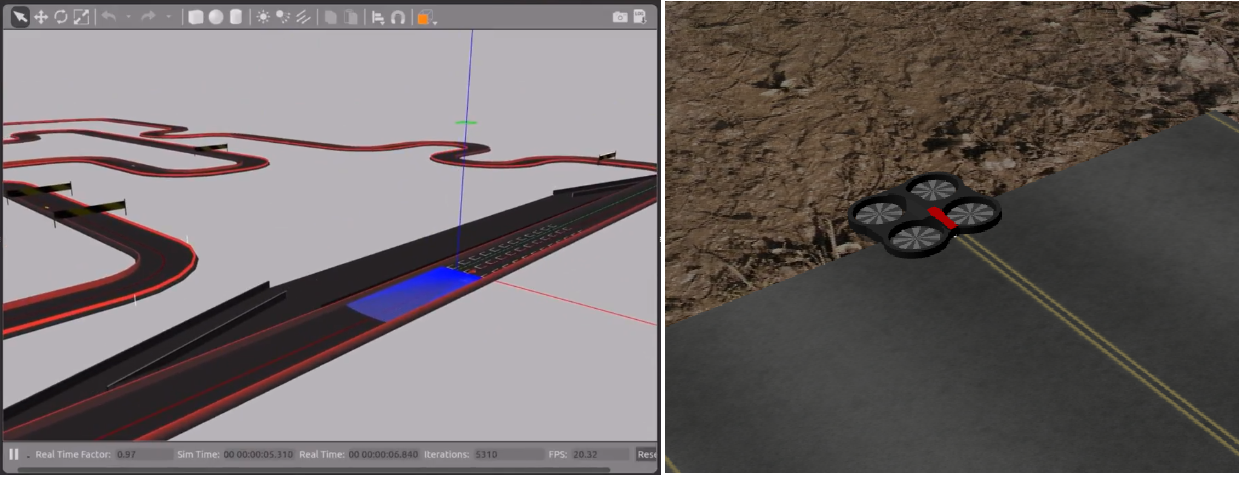
\includegraphics[width=0.9\linewidth]{figures/gazeboworlds.png}
		\caption{Ejemplo de mundo y modelo de Gazebo}
		\label{fig.worlds}
		\end{center}
\end{figure}

Los escenarios de Gazebo se describen en fichero con extensión ".world", que son ficheros escritos en XML (Extensible Remarkable Language) de descripción de documentos, definidos en el lenguaje de simulación SDF (Simulation Description Format), donde se recogen todos los elementos del escenario:

\begin{itemize}
	\item Escena: Iluminación, propiedades del cielo, sombras, etc.
	\item Mundo: Representación del mundo como conjunto de modelos, \textit{plugins} y propiedades físicas.
	\item Modelo: Componentes que forman el robot, como articulaciones, objetos de colisión, sensores, etc.
	\item Físicas: Gravedad, inercia, rozamiento, colisiones, motor físico, tiempo, etc.
	\item \textit{Plugins}: Pueden incluirse en el mundo, el modelo o un sensor. Pueden incluirse \textit{plugins} disponibles en la red como el que da soporte completo a la funcionalidad del robot Roomba, llamado \textit{libroombaplugin.so}.
\end{itemize}

Cada elemento del escenario cuenta con una etiqueta propia que lo distingue del resto. Cualquier propiedad descrita dentro de su etiqueta tiene que ir marcada con la etiquete de la propiedad correspondiente.
En la versión 7 de Gazebo se ha incluido un editor de modelos básico para poder desarrollar modelos y escenarios básicos. A partir de los modelos que se importen o desarrollen en Gazebo, es necesario adjuntar un \textit{plugin} que los dote de la funcionalidad necesaria, de otra manera no serían más que simples objetos inanimados.

\section{Editor de modelos}
Para el desarrollo del modelo de robots se ha trabajo con dos editores de modelos, SketchUp\footnote{\url{https://www.sketchup.com/}} y Blender\footnote{\url{https://www.blender.org/}}. Estos editores son necesarios para importar los modelos de robots generados en ellos al simulador Gazebo.
Existe un almacén web desde donde es posible descargarse una gran variedad de modelos y escenarios, además de desarrollar los propios. Una vez desarrollado el modelo o escenario, estos editores exportan el modelo o escenario en formato ".dae" (Digital Assets Exchange), formato perteneciente al lenguaje XML, y los correspondientes texturas en imágenes con formato ".JPG". Una vez obtenidos estos ficheros, ya son importables por el simulador Gazebo, pero es necesario una modificación para dotar al modelo o escenario de colisiones, inercias, gravedad, etc. 

Los escenarios y modelos generados por estos editores son creados mediante la intersección de líneas, generando los distintos tipos de objetos. Además, es posible adjuntar una textura o color a cada cara que forma el objeto. Además, el editor Blender, al ser más complejo, permite la introducción de iluminación y trabajar con formas geométricas en tres dimensiones directamente, en cambio el editor SketchUp trabaja con líneas, aunque es más sencillo de utilizar.

El editor de modelos Blender es de código abierto pero el editor de modelos SketchUp es de pago, pero tiene la ventaja de contar con su almacén de modelos en el que puedes descargar una gran variedad de modelos.

\section{Lenguaje Python}
Python\footnote{\url{https://www.python.org/}} es un lenguaje de programación orientado a objetos, interpretado y de alto nivel con semántica dinámica. Es un lenguaje de fácil aprendizaje y comprensión debido a su apariencia intuitiva. Su creador fue Guido van Rossum, un investigador holandés que trabajaba en el centro de investigación CWI (Centrum Wiskunde \& Informática. La primera versión de este lenguaje de programación surgió en 1991, pero no fue publicado hasta tres años después. El nombre que recibió este lenguaje fue dado por su creador en honor a la serie de televisión \textit{Monty Python's Flying Circus}.

La combinación del tipado y el enlace dinámico con sus estructuras de datos integradas de alto nivel, dotan a este lenguaje de un desarrollo rápido de aplicaciones, scripting o lenguaje de interconexión de componentes existentes. La sintaxis fácil y simple enfatiza su legibilidad y reduce el coste de mantenimiento del código. Además, Python admite módulos y paquetes, por lo que fomenta la modularidad del programa y la reutilización de código.

El intérprete de Python y la extensa biblioteca de paquetes están disponibles en formato binario o en código fuente de manera gratuita para las plataformas principales y pueden ser distribuidas libremente.

La última versión de Python Software Fundation es la 3.6.5. En este Trabajo de Fin de Grado hemos utilizado la versión 2.7.12, compatible con JdeRobot 5.6.2 y con ROS-Kinetic. De manera que la completitud de las dos prácticas desarrolladas en este trabajo está escrita en esta versión.

\section{Biblioteca OpenCV}
OpenCV\footnote{\url{https://opencv.org/}} (Open Source Computer Vision Library) es una librería de código abierto destinada al procesamiento de imágenes y el aprendizaje máquina. Fue desarrollada por Intel y publicada bajo licencia de BSD. El propósito de esta librería es facilitar el desarrollo de programas de visión por computador en tiempo real.

Se trata de una librería multiplataforma con soporte para MacOS, Linux, Android y Windows. Además, existen versiones en Java, Python y C\# a pesar de que era, originalmente, una librería en C/C++. También existen interfaces en desarrollo para Ruby, Matlab y otros lenguajes.
La librería OpenCV implementa algoritmos para técnicas de detección de rasgos, clasificación de acciones humanas en vídeos, reconocimiento, segmentación de objetos, calibración, seguimiento de caras, análisis de la forma y movimiento, reconstrucción 3D... Los algoritmo que componen esta librería están basados en estructuras de datos flexibles acoplados a estructuras IPL (\textit{Intel Image Processing Library}), utilizando la arquitectura de Intel respecto a la optimzación de la mayoría del paquete. También aprovecha la aceleración de cómputo gracias al uso de tarjetas gráficas avanzadas (GPUs). OpenCV fue desarrollado para tener una alta eficiencia computacional. Está escrito en el lenguaje de programación C y puede aprovechar las ventajas de los procesadores \textit{multicore} de nueva generación. Tales son las ventajas que aporta que las grandes compañías como Google, Yahoo, Microsoft, Intel, IBM, Sony, Toyota u Honda utilizan esta librería, que se ha convertido en el estándar de facto en su campo.

Para este trabajo se ha utilizado la librería OpenCV en la versión 3.2 y su ha sido empleada en toda la parte del código relacionada con tratamiento de imágenes.

\section{Biblioteca PyQt}
PyQt\footnote{\url{https://pypi.org/project/PyQt5/}} es un conjunto de enlaces Python utilizado para el conjunto de herramientas Qt, un \textit{framework} multiplataforma orientado a objetos y escrito en C++ que permite el desarrollo de interfaces gráficas. Incluye sockets, hilos, bases de datos SQL, Unicode, etc. Combina todas las ventajas de Qt y Python empleando todas las funcionalidades de Qt con un lenguaje de programación sencillo como es Python. Fue desarrollada por Riverbank Computing Ltd y tiene suporte multiplataforma con versiones para Windows, Linux, Mac OS X, iOS y Android.

Para este proyecto se ha utilizado la versión 5 de PyQt. Se trata de un conjunto de enlaces Python para Qt5, con soporte para Python 2.x y Python 3.x. Incluye más de 6000 funciones y 620 clases y métodos. Dispone de una licencia dual, es decir, puede elegirse una licencia comercial para usuarios o una licencia GPL (General Public Licence) para desarrolladores.
Las clases de PyQt5 se dividen en módulos: QtCore, QtGui, QtWidgets, QtXml y QtSql, entre otros. Para las prácticas desarrolladas, se han utilizado los siguientes módulos:
\begin{itemize}
	\item QtGui: contiene clases para la creación de interfaces gráficas y el desarrollo de gráficos en 2D, imágenes, texto y desarrollo de ventanas.
	\item QtCore: incorpora las clases principales no relacionadas con la interfaz gráfica. Se utiliza para trabajar con archivos, hilos, datos, procesos, urls, etc.
	\item QtWidgets: está formado por clases que proporcionan distintas funcionalidades a la interfaz del usuario.
\end{itemize}

\section{Jupyter}
Jupyter Notebook\footnote{\url{http://jupyter.org/}} se trata de una aplicación web de código abierto que permite al usuario desarrollar y compartir documentos que contengan código empotrado, ecuaciones, textos y visualizaciones. Proporciona una gran variedad de ventajas entre las que destacan limpieza, simulación numérica, modelado estadístico, visualización y transformación de datos, aprendizaje automático, etc. Inicialmente fue desarrollado como IPython 3.0 pero se renombró como Jupyter.

El cuadernillo de trabajo o \textit{Notebook} está compuesto por celdas en las que se inserta el código, en lenguaje Python, o distintos elementos de texto enriquecido como párrafos, ecuaciones, enlaces, figuras, etc. El resto de tipos de celdas son legibles para los humanos como figuras, tablas o texto y contienen los análisis y resultados del trabajo, además de documentos ejecutables para la ejecución del análisis.
El \textit{Notebook} está formado por una sucesión lineal de celdas. Hay cuatro tipos básicos:

\begin{itemize}
	\item \textbf{Celda de código}: se trata de input y output de código que se ejecuta en el kernel del cuadernillo a tiempo real.
	\item \textbf{Casillas de reducción}: son celdas de texto con ecuaciones en LaTex empotradas.
	\item \textbf{Encabezado de celdas}: formado por 6 niveles de organización jerárquica y su formato.
	\item \textbf{Celdas sin formato}: se trata de texto sin formato que se incluye en el cuadernillo sin ningún tipo de modificación cuando los cuadernillos son convertidos a formatos distintos mediante \textit{nbconvert}.
\end{itemize}

La aplicación tiene un modelo cliente-servidor que permite la ejecución y edición de los \textit{Notebooks} mediante un navegador web. La aplicación Jupyter puede ejecutarse desde un escritorio local sin necesidad de disponer de conexión a Internet o instalarse en un servidor remoto y acceder a ella a través de internet. Además de estas características, Jupyter dispone de un \textit{Panel de control} o llamado \textit{Dashboard} con el que permite la apertura, guardado y cierre de los archivos y los núcleos del \textit{Kernel}.

Estos \textit{kernels} son motores computacionales que ejecutan el código contenido en el \textit{Notebook}. Existen multitud de \textit{kernels} oficiales que dan soporte a distintos lenguajes como Python, Julia, R, Ruby Haskell, Scala, ...), incluso versiones distintas de \textit{kernels} para un mismo lenguaje. Al abrir el \textit{Notebook}, el \textit{kernel} se inicializa automáticamente. De este modo, al ejecutar una celda del cuadernillo se reproduce el código contenido en ella y, a continuación, de muestran los resultados. Es importante tener en cuenta que, dependiendo del código contenido en la celda, el \textit{kernel} puede consumir una gran cantidad de recursos CPU y RAM, que están limitados por el navegador.

Los cuadernillos, así como el resto de tipos de documentos (ficheros de código auxiliar, fichero de texto, imágenes, etc.) pueden guardarse y son almacenados en el sistema de fichero local del usuario. El \textit{Notebook} será almacenado con una extensión \textit{.ipynb} que puede ser ejecutado tras iniciar Jupyter.

Gracias a esta aplicación, se han desarrollado prácticas análogas a las existentes en la plataforma \textit{JdeRobot-Academy} en Jupyter. De esta manera, JdeRobot se acerca a dar soporte multiplataforma gracias al uso del navegador web y Jupyter para la interacción con su entorno docente. Para ello se ha empotrado el nodo académico de las prácticas en celdillas de un \textit{Noteboook} de Jupyter y se ha proporcionado una celdilla para que el alumno escriba el algoritmo de solución en él y sólo tenga que ejecutar esa celdilla para ver los resultados.
Los \textit{Notebooks} utilizados para la recreación de las prácticas han sido desarrollados en la versión 2.7 de Python, por lo que las prácticas y la solución que desarrollen los alumnos deben ser en esta versión.

\section{Academy-Web}
Esta plataforma web proporciona un servidor remoto para el desarrollo y ejecución de las prácticas contenidas en el entorno \textit{JdeRobot-Academy}. Esto supone una gran innovación y el paso final al soporte multiplataforma del entorno docente \textit{JdeRobot}.

Para ello se basa en el uso de Jupyter para cargar el nodo académico de las prácticas, así como de un script (incluido en el \textit{Notebook} de Jupyter) para realizar las conexiones de los sensores y actuadores del robot con el nodo académico. También utiliza el soporte del simulador Gazebo en navegadores web para ofrecer una visualización del escenario de la práctica cargando un fichero \textit{.world} donde se incluye la descripción del robot y el mundo. Para soportar esta carga computacional, el servidor de la plataforma está basado en el servidor \textit{Apache}\footnote{\url{https://www.apache.org/}}, sobre el que se ha desarrollado un servidor en  \textit{Django}\footnote{\url{https://www.djangoproject.com/}}. Ambas plataformas son de código libre y proporcionan el código necesario para el desarrollo de servidores web. Por último, utiliza \textit{Dockers}\footnote{\url{https://www.docker.com/}} para ofrecer al estudiante todos los componentes necesarios para dar soporte a toda la infraestructura anterior. De esta manera, tanto JdeRobot, ROS-Kinetic, modelos, escenarios, \textit{plugins}, \textit{drivers}, etc. Están disponibles y son totalmente transparentes al alumno.

Mediante la integración de todas las plataformas anteriores se ha conseguido desarrollar el servidor web \textit{Academy-Web} que proporciona al estudiante todas las herramientas necesarias para realizar las prácticas que contiene en cualquier plataforma de una manera muy sencilla. el servidor ofrece la visualización del escenario en Gazebo junto con el cuadernillo de Jupyter en el que está presente la celda en la que el estudiante desarrollará su código (Figura 3.2).

\begin{figure}[H]
  \begin{center}
    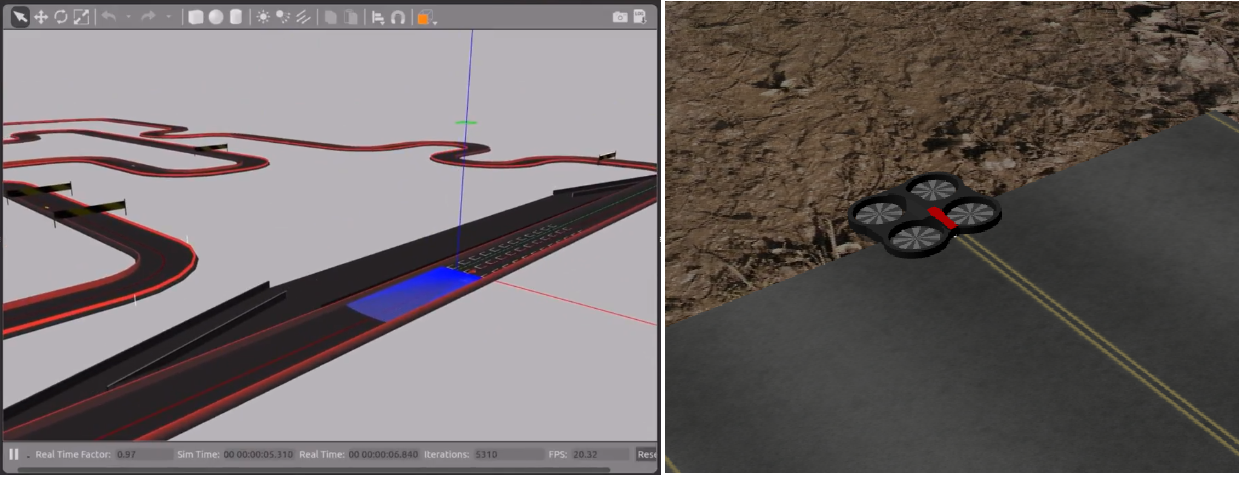
\includegraphics[width=0.9\linewidth]{figures/gazeboworlds.png}
		\caption{Visualización de la práctica XXXXX en Academy-Web}
		\label{fig.academyweb}
		\end{center}
\end{figure}

